%%%%%%%%%%%%%%%%%%%%%%%%%%%%%%%%%%%%%%%%%%%%%%%%%%%%%%%%%%%%%%%%%%%%
%% I, the copyright holder of this work, release this work into the
%% public domain. This applies worldwide. In some countries this may
%% not be legally possible; if so: I grant anyone the right to use
%% this work for any purpose, without any conditions, unless such
%% conditions are required by law.
%%%%%%%%%%%%%%%%%%%%%%%%%%%%%%%%%%%%%%%%%%%%%%%%%%%%%%%%%%%%%%%%%%%%

\documentclass[
  12pt, 
  digital, %printed, %digital, %% This option enables the default options for the
           %% digital version of a document. Replace with `printed`
           %% to enable the default options for the printed version
           %% of a document.
  notable,   %% Causes the coloring of tables. Replace with `notable`
           %% to restore plain tables.
  nolof,     %% Prints the List of Figures. Replace with `nolof` to
           %% hide the List of Figures.
  nolot,     %% Prints the List of Tables. Replace with `nolot` to
           %% hide the List of Tables.
  %% More options are listed in the user guide at
  %% <http://mirrors.ctan.org/macros/latex/contrib/fithesis/guide/mu/fi.pdf>.
]{fithesis3}
%% The following section sets up the locales used in the thesis.
\usepackage[resetfonts]{cmap} %% We need to load the T2A font encoding
%\usepackage[T1,T2A]{fontenc}  %% to use the Cyrillic fonts with Russian texts.
\usepackage[
  main=english, %% By using `czech` or `slovak` as the main locale
                %% instead of `english`, you can typeset the thesis
                %% in either Czech or Slovak, respectively.
  slovak %% The additional keys allow
]{babel}        %% foreign texts to be typeset as follows:
%%
%%   \begin{otherlanguage}{german}  ... \end{otherlanguage}
%%   \begin{otherlanguage}{russian} ... \end{otherlanguage}
%%   \begin{otherlanguage}{czech}   ... \end{otherlanguage}
%%   \begin{otherlanguage}{slovak}  ... \end{otherlanguage}
%%
%% For non-Latin scripts, it may be necessary to load additional
%% fonts:
\usepackage{paratype}
\def\textrussian#1{{\usefont{T2A}{PTSerif-TLF}{m}{rm}#1}}
%%
%% The following section sets up the metadata of the thesis.
\thesissetup{
    date          = 2017/06/04, %\the\year/\the\month/\the\day,
    university    = mu,
    faculty       = fi,
    type          = bc,
    author        = Lenka Svetlovská,
    gender        = f,
    advisor       = {RNDr. Andriy Stetsko, Ph.D.},
    title         = {Security and cryptography in GO},
    TeXtitle      = {Security and cryptography in GO},
    keywords      = {Certificate, Cgo, Language C, Language Go, OpenSSL, Pre-shared key, Security, TLS, TLS\_PSK},
    TeXkeywords   = {Certificate, Cgo, Language C, Language Go, OpenSSL, Pre-shared key, Security, TLS, TLS\_PSK},
    bib           = example.bib,
}
\thesislong{abstract}{
The main goal of this bachelor thesis is an implementation of an application able to connect to a 
server using pre-shared key cipher suite, communicate with server and support of X.509 certificates, 
such as generation of asymmetric keys, certificate signing request and different formats. The 
application is implemented in language Go.

The very first step involves looking for suitable Go library which can connect to a server using pre-shared key cipher suite, and work with cryptography and X.509 certificates. The thesis contains the overview, comparison, and evaluation of existing cryptographic Go libraries.
}
\thesislong{thanks}{
I would like to thank RNDr. Andriy Stetsko, Ph.D. for the management of the bachelor thesis, 
valuable advice, and comments. I would also like to thank the consultant from Y Soft Corporation 
a.s., Mgr. Lenka Bačinská, for useful advice, dedicated time and patience in consultations and 
application development. 

Likewise, I thank my family and friends for their support throughout my studies and writing this 
thesis.
}
\usepackage{makeidx}      %% The `makeidx` package contains
\makeindex                %% helper commands for index typesetting.
%% These additional packages are used within the document:
\usepackage{paralist} %% Compact list environments
\usepackage{amsmath}  %% Mathematics
\usepackage{amsthm}
\usepackage{amsfonts}
\usepackage{url}      %% Hyperlinks
\usepackage{markdown} %% Lightweight Markup

%added usepackages
\usepackage{rotating} %rotate table
\usepackage{longtable} %rozdelit tabulku na viac stran

\usepackage[table]{xcolor}
\usepackage{array}
%\definecolor{myColor}{RGB}{255,240,240} %pink
\definecolor{myColor2}{rgb}{0.95,0.95,0.92}%{RGB}{233,233,233} %grey
\usepackage[flushleft]{threeparttable} %note in table
\newcolumntype{P}[1]{>{\centering\arraybackslash\columncolor{myColor2}}m{#1}} %grey{E9E9E9}
\newcolumntype{Q}[1]{>{\centering\arraybackslash}m{#1}}

\usepackage{enumitem}
\usepackage{graphicx,lipsum,wrapfig} %obrazok obtekany textom
\usepackage{footnote}
\usepackage{listings} %programovacia cast + nasledovne nastavenia
\usepackage{color}
%New colors defined below
\definecolor{codegreen}{rgb}{0,0.6,0}
\definecolor{codegray}{rgb}{0.5,0.5,0.5}
\definecolor{codepurple}{rgb}{0.58,0,0.82}
\definecolor{backcolour}{rgb}{0.95,0.95,0.92}
%Code listing style named "mystyle"
\lstdefinestyle{mystyle}{
  backgroundcolor=\color{backcolour},   commentstyle=\color{codegreen},
  keywordstyle=\color{magenta},
  numberstyle=\tiny\color{codegray},
  stringstyle=\color{codepurple},
  basicstyle=\footnotesize,
  breakatwhitespace=false,         
  breaklines=true,                 
  captionpos=b,                    
  keepspaces=true,                 
  numbers=left,                    
  numbersep=5pt,                  
  showspaces=false,                
  showstringspaces=false,
  showtabs=false,                  
  tabsize=2
}
%"mystyle" code listing set
\lstset{style=mystyle}

\usepackage{verbatim} %comment
 %subfigure
\usepackage{caption}
\usepackage{subcaption}


\begin{document}
\chapter{Introduction}
\begin{comment}
One of the oldest systems of symmetric cryptography is probably \textit{“Skytale”} used in 5th 
century BC. 
A secret was made by a stick with some diameter which was reeled leather stripe on so that 
covered surface of the stick. A message was written there, and after the untangled, the text was 
unreadable. Cryptography informs as we know nowadays, it began to develop at the beginning of 20th 
century especially with development telegraphs. Using cryptography happened necessary part of 
ordinary life. All connections through we communicate are secured by some case through 
cryptographic functions. An~only little mistake in those functions can cause to misuse private 
data. 
\end{comment}    
Programming language Go is a general-purpose, compiled and statically typed language with garbage 
collection and safety memory features. Language Go was made by Google Inc. company in 2007, and its 
syntax is derived from language C. Safety, speed and concurrency are its main characters. Go 
provides extensive options for cryptography, such as encryption, hashing and work with 
certificates. 

The main aim of this bachelor thesis is an implementation of an~application in language Go. The 
application will be able to connect to a~server using pre-shared key cipher suite and communicate with 
it. The~application will also support of X.509 certificates, such as generation of asymmetric keys, certificate signing request in different formats which are described in subsection \ref{formats}. 

First, it is necessary to examine features of language Go related to security and cryptography what 
involves looking for suitable Go library. Go library should connect to a server using pre-shared key 
cipher suite, and work with cryptography and X.509 certificates. 

The thesis contains the overview, evaluation, and comparison of existing cryptographic libraries based 
on their license, usability, supported cryptographic functions, such as symmetric and asymmetric 
encryption and hash functions. Next, based on possibilities to generate cryptographic keys, support for 
SSL/TLS protocol, generation of certificate signing requests, and support for different formats and 
extensions. The thesis also contains the implementation, tests, and evaluation of the application.

The bachelor thesis is consulted and realized in collaboration with Y~Soft~Corporation,~a.s.


\chapter{Background}
In this chapter, I will define the basic terms which are necessary for understanding of a 
text presented in the following sections. First I~will describe a structure of certificates, 
standard X.509, certificate authority and signing process. I will explain self-signed certificate 
and formats of certificate view. Finally, I will describe protocols SSL/TLS and TLS pre-shared key 
(TLS\_PSK) algorithm used in the application.

\begin{comment}

\section{Cryptography}
Cryptography is the study of mathematical techniques related to aspects of information
security such as confidentiality, data integrity, entity authentication, and data origin
authentication \cite{menezes1996handbook}.Today we talk about computer security which consists 
in the fact that the attacker does not have enough computational strength and time to decode 
the cipher.

\subsection{Symmetric Cryptography}
Symmetric encryption, as the name suggests, means that the encryption and decryption of 
plaintext are based on sharing a together secret - keys.
Symmetric ciphers could be divided into block and stream. Stream ciphers encrypt each 
character of plaintext separately, usually one bit. Block ciphers encrypt plaintext into 
blocks with fixed bit length \textit{n}.

The main disadvantage of symmetric cryptography is the necessity of a large number of keys 
and need of their distribution. For example, for together communication \textit{n} operators 
need to have \[ \frac{n * (n - 1)}{2}\] keys. It means that for the encrypted communications 
of mid-size company with 50 employees, it would need to share 1225 different keys. 

On the other hand, the advantage is the low computational complexity of symmetric ciphers. 
Their using is also useful in cases where the encrypted data are not sent anywhere, for 
example, to protect files on a personal computer.
 
\subsection{Asymmetric Cryptography}
Asymmetric cryptography allows data encryption and particularly the implementation of the 
digital signature. Each entity has two keys. The first is the private key that is used to 
decrypt a message or create a digital signature. It must be kept secret. The second key is 
public which is used for encryption and authentication of the digital signature. Of course, 
there is impossible to derive the private key from the public key \cite{dostalek2016velky}.

The main advantages of asymmetric cryptography are mainly a smaller number of keys than 
symmetric cryptography. If each entity has one public and one private key, it means that for 
\textit{n} entities are needed \textit{2n} keys. In the same situation as in the previous 
example, a company of 50 employees would need to ensure the safety of 100 keys, which is 
substantially less than 1225.

The biggest disadvantage of asymmetric cryptography is its slowness compared with symmetric 
cryptography. Therefore, they are most often used together, while the text is encrypted with a 
random symmetric encryption key. The key is encrypted using asymmetric ciphers. In the case of 
a digital signature, the first is created the fixed length hash of the message and then it is 
signed using asymmetric cryptography.

\subsection{Hash Function}
Hash functions are one of the basic elements of modern cryptography, often called one-way 
hash function.

Hash functions are effectively designed display binary strings unlimited length to binary 
strings a fixed length, called hash value. For a perfect hash function that has \textit{n}-bit 
hash value, there is a chance that a randomly selected string will be displayed on specific 
hash value $2^{-n}$. The basic idea of hash functions is that the hash value should serve as a 
representative of the input string. Hash function suitable for use in cryptography is usually 
chosen so that it is computationally very difficult find two different input strings that have 
the same hash value. If it succeeds in these two find strings, we say that we found a 
collision. 
Likewise, it should be computationally very difficult to find for a hash value corresponding 
to the input string. Using hash functions are used frequently to check the integrity of data 
and for digital signing of data \cite{piper2006kryptografie}.

\end{comment}

\section{Certificate}
The certificate is digitally signed data structure which contains a~public key of certificate 
owner. There are some standards of~the~certificate structure (X.509 (see subsection \ref{x509}), EDI - Electronic Data Interchange \cite{edi}, WAP - Wireless Application Protocol \cite{sharma2003wireless}, etc.). On the~Internet the mostly used standard is X.509 version 3, 
which was issued by ITU \cite{dostalek2016velky}. %For the needs of the Internet, there is created an Internet profile of X.509 in the relevant RFC. Current Internet profile certificate is standard RFC-5280 \cite{dostalek2016velky}.

\subsection{Standard X.509}\label{x509}
Standard X.509 was originally designed as an authentication framework for X.500 directories. They 
have a hierarchical structure, and the~individual attributes can be assigned to specific computers 
of companies or individual printers. Each entity can be clearly identified, and each has its 
private and public key \cite{schmeh2006cryptography}. 

An X.509 certificate, shown in figure \ref{fig:certificate}, contains information about the~identity to which a certificate is issued and the identity that issued it. 

The first version was very simple and nowadays it is already inadequate. It contained 7 fields:
\begin{itemize}[leftmargin=2em,rightmargin=1em,itemsep=0.75\parskip,parsep=0em,topsep=0em,partopsep=0em]
\item certificate version;
\item certificate series number;
\item algorithm which signed certificate;
\item name of certificate authority which released the certificate;
\item identity of certificate owner;
\item public key of certificate owner;
\item certificate validity.
\end{itemize}
\vskip 0.1in

Two new fields were added to the second version:
\begin{itemize}[leftmargin=2em,rightmargin=1em,itemsep=0.75\parskip,parsep=0em,topsep=0em,partopsep=0em]
\item unique identifier of the certificate owner;
\item unique identifier of the certificate authority.
\end{itemize}
\vskip 0.1in

The third version was introduced in 1996. Its biggest and most important benefit is support of
the extension. It eliminates the majority of shortcomings of previous versions 
\cite{housley2002internet}. 

An extension field permits any number of additional fields to be added to the certificate. 
Certificate extensions provide a way of adding information such as alternative subject names and 
usage restrictions to certificates \cite{b.3}.

\begin{figure}[th]
	\centering
	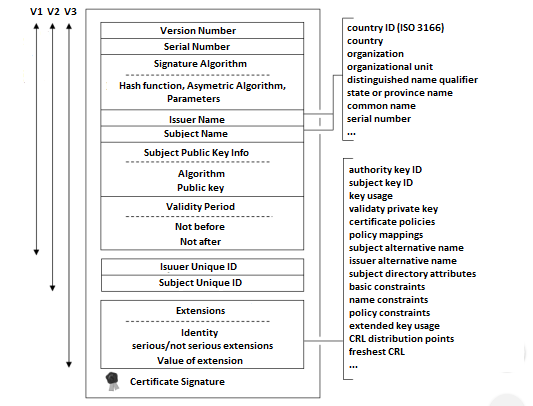
\includegraphics[width=1\textwidth]{certificate}
	\caption{Structure of X.509 Certificate; translated from \cite{ostadal_2010}}
	\label{fig:certificate}
\end{figure}

\subsection{Certificate Authority}
The Certificate Authority (CA) is an independent third party which issues certificates.

The CA arose to ensure secure encryption through a~certified public key and guarantee the validity 
of a digital signature \cite{singh2003kniha}. The CA also inspects a certificate request and 
provides validity revocation of certificate. In order to be truly credible, the CA must be 
impartial and, if it is possible, subordinate to some higher CA. Subordination means that it 
identifies the usage of certificates signed by a higher certificate authority 
\cite{dostalek2016velky}.

Root CAs, certificate authorities at the highest level, use a certificate signed by themselves 
(self-signed certificate).

\subsection{Self-signed Certificate}
The self-signed certificate is a certificate which the owner issues by himself. The self-signed 
certificate has a same data structure as a~regular certificate issued by CA. This certificate can 
be recognized by equality of Subject and Issuer items.

As proof of a private key possession, the self-signed certificate uses a digital signature which 
was made using the private key belonging to a public key in the certificate. Verification of 
the~signature is carried out through a public key in the actual 
certificate~\cite{dostalek2016velky}.

\begin{comment}
Self-signed certificate is used by software internally. While the applicant generates CSR to 
be issued by the CA, the public key must be kept by the applicants. In this case, the public 
key is often maintained like a self-signed certificate. Subsequently it is rewritten by the 
certificate.
\end{comment}

\subsection{Certificate Signing Request}
The certificate applicant can request CA to sign a certificate by submitting a data structure called 
a certificate signing request (CSR). The~most common format is PKCS\#10 \cite{dostalek2016velky}. The 
CSR should include:
\begin{itemize}[leftmargin=2em,rightmargin=1em,itemsep=0.75\parskip,parsep=0em,topsep=0em,partopsep=0em]
\item Applicant ID
\item Public key
\item Evidence of the possession of the private key
\item Other information that the owner wishes to insert in certificate
\item May contain evidence of the data generation
\item Data necessary for billing (in case issuance of certificates is paid)
\item Passwords for communication with CA:
  \begin{itemize}[leftmargin=2em,rightmargin=1em,itemsep=0.75\parskip,parsep=0em,topsep=0em,partopsep=0em]
  \item One-time password for issuing the certificate
  \item One-time password for certificate revocation
  \item Permanent password for personal (non-electronic) communication between owner and CA
  \item Phrase (useful in case losing all passwords; for example mother's maiden name) 
  \end{itemize}
\end{itemize} 

A certificate authority must fill individual fields of the certificate before it signs a 
result digitally. The CA takes CSR, checks completed fields, and fills two important fields 
the time period, represented by not before and not after attributes, in which the certificate is 
valid. The CA can also add extensions, such as Subject Alternative Name, information 
about CA, etc. (shown in figure \ref{fig:certificate}) \cite{dostalek2016velky}.

\subsection{Formats PEM and DER}\label{formats}
The PEM (Privacy Enhanced Mail) is  file format for storing and sending cryptographic keys, 
certificates, and other data. It is designed to be secure for inclusion in ASCII or even rich-text 
documents. This means that it is easy to copy and paste a content of a PEM file to another 
document and back \cite{howToSsl}. The following figure, \ref{fig:vzorPEM-DER}, is a~sample PEM 
file containing a private key and a certificate. 

\begin{figure}[th]
	\centering
	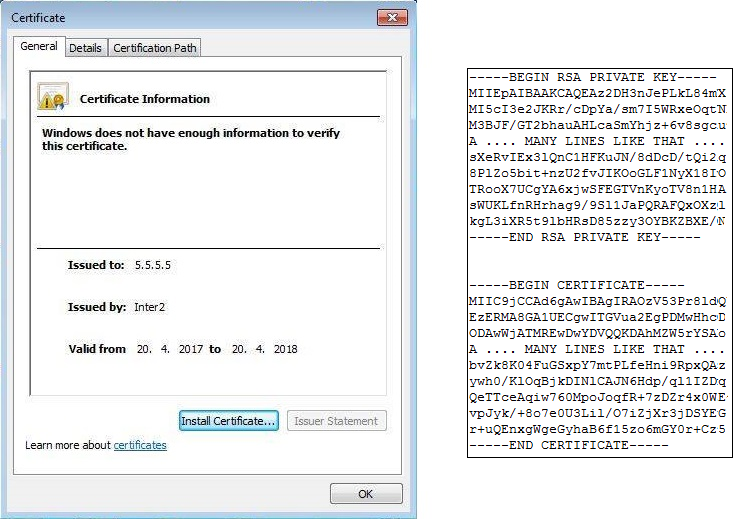
\includegraphics[width=0.83\textwidth]{pem-der-fig}
	\caption{An example of certificate view}
	\label{fig:vzorPEM-DER}
\end{figure}

\begin{comment}
\begin{figure}
\centering
\begin{subfigure}[b]{0.6\textwidth}
  \centering
  \includegraphics[width=0.9\linewidth]{win-cert}
  \caption{A subfigure}
  \label{fig:sub1}
\end{subfigure}
\begin{subfigure}[b]{0.2\textwidth}
  \centering
  \includegraphics[width=0.9\linewidth]{pem-key-cert}
  \caption{A subfigure}
  \label{fig:sub2}
\end{subfigure}
\caption{A figure with two subfigures}
\label{fig:test}
\end{figure}
\end{comment}
A certificate or key must start with a header where the number of dashes is important and must be 
correct. 

The certificate starts with: "- - - - -BEGIN CERTIFICATE- - - - -" and ends with: "- - - - -END CERTIFICATE- - - - -". 

The key, for example RSA private key, starts with: "- - - - -BEGIN RSA PRIVATE KEY- - - - -" and ends 
with: "- - - - -END RSA PRIVATE KEY- - - - -". 

A single PEM file may contain more certificates or keys, for example, it is possible to have a single file with public certificate, intermediate certificate, root certificate and private key.

The DER (Distinguished Encoding Rules) is a binary form of ASCII PEM format certificate. DER is used 
to represent keys, certificates and such in a portable format. All types of certificates and private 
keys can be encoded in DER format. Its information is stored in a binary DER for ASN.1 \cite{asn.1}. 
Applications providing RSA, SSL and TLS should handle DER encoding to read an information \cite{bakker_2014}. %DER can not contain more than one certificate or one key.

\section{Protocol SSL/TLS}
Protocol SSL/TLS is used for secure communication between a~client and a server. Protocol SSL was 
developed by Netscape Communications which published three versions. The first version was only 
a~test; the second has been used in practice. However, it still contained security vulnerabilities; 
the most important was susceptibility to attack \textit{man in the middle} \cite{oppliger2003security}. The third version was introduced in 1996, and its specification could 
be found in the document \textit{The SSL Protocol Version 3.0} (SSLv3.0) \cite{freier2011secure}. 

TLS protocol was created from \textit{SSLv3.0} and it is currently the most widespread and 
supported protocol \cite{oppliger2003security}. There are currently three versions which have only 
minimal differences (for more details see \cite{differences}). \textit{TLS version 1.3} (TLSv1.3) 
is a draft already used in multiple locations \cite{draft-tls}. For example, the forthcoming \textit{OpenSSL 1.1.1} release will include support for \textit{TLSv1.3} \cite{foundation2}.

Protocol SSL/TLS provides authentication of two communicating parties by using asymmetric 
encryption, message integrity by using MAC and confidentiality by encrypting all communications 
by selected symmetric cipher.

Protocol SSL/TLS is located between the application and a transport layer reference ISO/OSI model 
and consists of two main parts. Those parts are \textit{The Record Layer Protocol} and \textit{Handshake Protocol} \cite{oppliger2003security}. %Part of HP are two auxiliary protocols - \textit{Change Cipher Specification Protocol} (CCSP) and \textit{Alert Protocol} (AP) \cite{oppliger2003security}.

\subsubsection{Record Layer Protocol (RLP)}

RLP processes application data, performs fragmentation, compression and data encryption. Moreover, it also decrypts data and verifies the~checksums. RLP does not care about type of an encryption algorithm or encryption key setting. This information is given by HP~\cite{oppliger2003security}.

\subsubsection{Handshake Protocol (HP)}
HP is activated immediately after establishment of a connection and provides identification of 
communicating parties, negotiation of cryptographic algorithms, compression algorithms and other 
attributes. Then it creates a \textit{master secret}, from which encryption keys are derived, 
initialization vectors, and the MAC (Message Authentication Code)~\cite{oppliger2003security}. 

A client and a server use asymmetric encryption to generate a shared secret key. The shared key is used 
for the symmetric encryption of messages because it is faster than asymmetric encryption \cite{ibm}. 

\begin{figure}[th]
	\centering
	\includegraphics[width=1.05\textwidth]{tls-hs-static-rsa}
	\caption{TLS handshake \cite{tls-fig}}
	\label{fig:tls}
\end{figure}

The figure \ref{fig:tls} illustrates TLS handshake. In nutshell, the steps involved in  the SSL/TLS handshake are as follows:

\begin{enumerate}
\item The client sends a \textit{ClientHello} message to a server, along with TLS version, supported cipher suites and a~client's random value.
\item The server responds by sending a \textit{ServerHello} message that contains the cipher suite chosen from the list which is provided by the client, server's random value, and the session ID. 
\item The server sends its digital certificate to the client and may request a certificate from the client. Then the server sends the \textit{ServerHelloDone} message.
\item The server sends a "Client certificate request" when requires a certificate for a client authentication. The client responds with its certificate.
\item 
\begin{enumerate}
\item The client creates a \textit{Pre-Master Secret} randomly and encrypts it with the server's public key. Encrypted \textit{Pre-Master Secret} is then sent to server. 
\item The server and client generate random values, exchange them and both create \textit{Pre-Master Secret}.
\end{enumerate} 
\item The server and the client both generate the \textit{Master Secret} and session keys from the \textit{Pre-Master Secret}.
\item The client sends \textit{ChangeCipherSpec} notification to server. It indicates that the client starts to use the new session keys for encrypting messages. Client also sends \textit{ClientFinished} message.
\item Server receives \textit{ChangeCipherSpec} and prepares to use the session keys for symmetric encryption. Server sends \textit{ServerFinished} message to the client.
\end{enumerate}

Client and server established the secured channel. Now, they can exchange application data over this channel. All messages sent from server to client and from client to server are encrypted by session key~\cite{ibm, handshakeprotocol}.

\begin{comment}
\begin{enumerate}
\item The client wants to connect to the server and sends \textit{ClientHello}, which contains 
the highest number of version supported by SSL/TLS, the number of session (it is empty if it 
is a new session), the list of supported ciphers and compression methods and a random number.
\item The client waits for a response in the form of a report \textit{ServerHello}, which will 
contain the highest number of versions of SSL/TLS, which is supported by server and client. It 
will also contain encryption and compression method, which are selected from the list received 
in step one, a random number and its public key certificate (the server can also request 
client authentication).
\item The client validates the server certificate and sends a request to exchange keys. At the end the server and client share a common \textit{premaster secret}. \textit{The master secret} is derived from it. The \textit{ClientHello} and \textit{ServerHello} are derived from the master secret.
\item From this moment, the communication has been encrypted and the client sends a message that ends with this phase. In case the server required the client authentication, it has been carried out in this step. Finally, the server sends a confirmation used ciphers and message about the completion of this phase, thereby HP ends.
\end{enumerate}
\end{comment}

%\textit{Change Cipher Specification Protocol} is a simple protocol that contains only a single message. It says there was the change of the encryption parameters and now only new ones will be used. It could be also called after the end of the initial phase.

%\textit{Alert protocol} provides the transmission of warning in case of any problem in communication - it contains an array of warning severity and description of the problem.

\begin{comment}
TLS uses public key certificates for authentication. To establish a TLS connection are used 
symmetric keys (later called pre-shared keys or PSKs), shared in advance among the 
communicating parties \cite{eronen2005pre}.
\end{comment}

\subsection{PSK Key Exchange Algorithm}\label{pskAlgorithm}
Using pre-shared keys can, depending on the cipher suite, avoid the~need for public key operations.  This is useful if SSL/TLS is used in performance-constrained environments with limited CPU power.

Pre-shared keys may be more convenient from a key management point of view.  For instance, in closed environments where the connections are mostly configured manually in advance, it may be easier to configure a PSK than to use certificates. Another case is when the parties already have a mechanism for setting up a shared secret key, and that mechanism could be used to "bootstrap" a key for authenticating a TLS connection.

The cipher suites with PSK exchange algorithm use only symmetric key algorithms. Figure \ref{fig:psk} illustrates the pre-shared key algorithm.

\begin{enumerate}
\item The client indicates to use pre-shared key authentication by including one or more PSK cipher suites in the \textit{ClientHello} message. 
\item If the TLS server also wants to use pre-shared keys, it selects one of the PSK cipher suites and places it in the \textit{ServerHello} message. 
\item The server can provide a PSK identity hint\footnote{In a PSK exchange algorithm, both the client and the server have to be able to derive the same set of cryptographic keys. The identity hint is something the server provides to tell the client how to derive the key \cite{eronen2005pre}.} in the~\textit{ServerKeyExchange} message. If no hint is provided, the~\textit{ServerKeyExchange} message is omitted.
\item The client indicates which key to use by including a PSK identity in the~\textit{ClientKeyExchange} message.
\item A \textit{Certificate} and \textit{CertificateRequest} payloads are omitted from the~response.
\item The TLS handshake is authenticated using the \textit{Finished} messages. 
\end{enumerate}

\begin{figure}[th]
	\centering
  	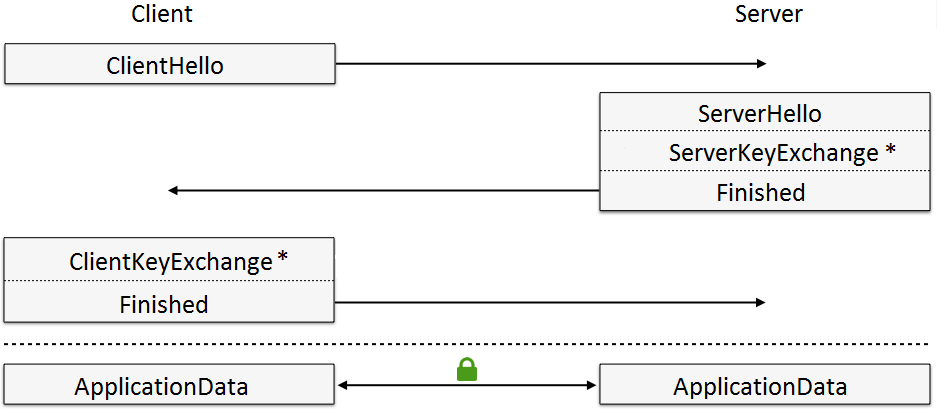
\includegraphics[width=1.05\textwidth]{psk-edited}%{tls13-hs-resumption}%{psk}
   \caption{TLS\_PSK Key Exchange; edited from \cite{taubert}}
   \label{fig:psk}
\end{figure}

If the server does not recognize the PSK identity, it may respond with an \textit{unknown\_psk\_identity} 
alert message. Alternatively, if the server wishes to hide the fact that the PSK identity was not known, 
it may continue the protocol as if the PSK identity existed, but the key was incorrect: it means to 
respond with an \textit{decrypt\_error alert} later \cite{eronen2005pre}. 

\subsubsection{Diffie-Hellman PSK}
Cipher suites which are using Diffie-Hellman with pre-shared key (DHE\_PSK) exchange algorithm are using 
PSK to authenticate a~Diffie-Hellman exchange. These cipher suites give some additional protection 
against dictionary attacks by passive eavesdroppers (but not active attackers) and also provide Perfect 
Forward Secrecy \cite{pfs}.

When these cipher suites are used, the \textit{ServerKeyExchange} and \textit{ClientKeyExchange} messages 
also include the Diffie-Hellman public parameters. The PSK identity and identity hint fields have the 
same meaning as in the previous algorithm, but in DHE\_PSK algorithm the \textit{ServerKeyExchange} 
message is always sent, even if no PSK identity hint is provided \cite{eronen2005pre}.

DHE\_PSK are present since \textit{OpenSSL} version 1.1.0.
%zdroj https://www.openssl.org/news/changelog.html

\chapter{Language Go}\label{go}
In this chapter, I will explain the main characteristics of language Go and show how to write the 
code. Next, I will describe Go libraries called packages and the tool Cgo.

\section{Introduction}
Go is a programming language developed by \textit{Google} in the year 2007 and announced in 
November 2009. Many companies have started using Go because of its performance, simplicity, 
ease of use and powerful tooling \cite{doxsey2016introducing}. Go programming language is a 
statically-typed language with advanced features and a clean syntax. It is compiled language like \textit{C++} and a dynamic language like \textit{Python} \cite{harris_2015}. It provides:
\vskip0.1in
\begin{itemize}[leftmargin=2em,rightmargin=1em,itemsep=0.75\parskip,parsep=0em,topsep=0em,partopsep=0em]
\item garbage collector - memory is cleaned up automatically when nothing refers to it 
anymore,
\item fast compilation time - through effective work with individual parts of a program and simple grammar,
\item light-weight processes (via go-routines), channels,
\item a rich standard library,
\item easy testing - incorporated directly into the core language,
\item clear documentation full of examples.
\end{itemize}
\vskip0.1in

Go excluded some features intentionally to keep language simple and concise. There is no 
support for type inheritance, method or operator overloading, circular dependencies among 
packages, pointer arithmetic, assertions or for generic programming \cite{doxsey2016introducing, wiki-go}.

\section{How to Start}\label{howToStart}
This section contains short instructions how to start with Go programming language, what to install, set it up and how to compile and run programs.

\subsection{Installation}
Golang \footnote{https://golang.org/dl/}, the Go official website, provides an installer of Go to 
download free binaries release suitable for Windows, Linux, Mac OS X and FreeBSD. On Windows 
system, Go is installed simply by opening MSI file and following the installation guide. By default, the installer puts the Go distribution in $C:\backslash Go$. 

It is even easier to install Go via package managers, for example on Debian based system, for example:
\begin{lstlisting}
sudo apt-get install golang
\end{lstlisting}
%To confirm everything is working, open a terminal and type the following:
%\begin{lstlisting}
%go version
%\end{lstlisting}
Upgrading from an older version of Go must be predecessed by removing an existing version. 

\subsection{Environment}
After installation, it is necessary to create \textit{\$GOROOT} environment variable with Go location directory and also add Go binary location to \textit{\$PATH} environment variable. The Go 
toolset uses an environment variable called \textit{\$GOPATH} to find Go source code. 

%For example, if you installed Go to your home directory you should add commands like the following to \textit{\$HOME/.profile}:
%Set up your workplace, for example \textit{GOPATH=C:/Projects/Go}.
\begin{lstlisting}
export GOROOT=/path/to/go1.X
export PATH=$PATH:$GOROOT/bin
export GOPATH=$HOME/Projects/go
\end{lstlisting}
Go typically keep all code in a single workspace. A workspace contains many version control 
repositories (managed by Git, for example). Each repository contains one or more packages and each 
package consists of one or more Go source files in a single directory. The path to a~package's 
directory determines its import path \footnote{This differs from other programming environments in 
which every project has a~separate workspace and workspaces are closely tied to version control 
repositories~\cite{howtowritegocode}.}. A workspace is a~directory hierarchy with three 
directories: \textit{src} contains Go source files, \textit{pkg} contains package objects, and \textit{bin} contains executable files~\cite{howtowritegocode}. %\textit{\$GOPATH} has to contain directories \textit{src} and \textit{pkg}.

\begin{comment}
\subsection{First Program}
Traditionally, the first program in any programming language is called a
hello program — a program that simply outputs "Hello World!" to terminal.

Open text editor, create file $hello.go$, and enter the following:
\begin{lstlisting}
package main
import "fmt"
// this is a comment
func main() {
	fmt.Println("Hello World!")
}
\end{lstlisting}
Make sure the file is identical to what is shown here and save it.
\end{comment}

\subsection{Compilation and Arguments}
Go is a compiled language, and like many languages, it makes heavy use of the command line. The following command compiles and runs program:
\begin{lstlisting}
go run <file-name>.go
\end{lstlisting}
The following command parameterizes execution of programs. First must be used \texttt{go build} command to create a binary program.
\begin{lstlisting}
go build <file-name>.go
./<file-name> <arguments>
\end{lstlisting}
In code below, $os.Args$ provides access to raw command-line arguments. The~first value is a path to the program, and \textit{os.Args[1:]} holds the~arguments to the program.
\begin{lstlisting}
argsWithProg := os.Args
argsWithoutProg := os.Args[1:]
arg := os.Args[3]
\end{lstlisting}
Here is necessary to import package $os$.

\begin{comment}
\subsection{Arguments}
Command-line arguments are a common way to parameterize execution of programs. First must be used go build command to create a binary program.
\begin{lstlisting}
go build cmd-arguments.go
./cmd-arguments a b c
\end{lstlisting}
In code, $os.Args$ provides access to raw command-line arguments. The first value is the path to the program, and \textit{os.Args[1:]} holds the arguments to the program.
\begin{lstlisting}
argsWithProg := os.Args
argsWithoutProg := os.Args[1:]
arg := os.Args[3]
\end{lstlisting}
Do not forget to import package $os$.
\end{comment}

\section{Packages}
In Go, source files are organized into system directories called packages. To  develop 
software applications, writing maintainable and reusable pieces of code is very important. Go 
provides the modularity and code reusability through its package system. Go encourages 
programmers to write small pieces of software components through packages, and compose their  
applications with these small packages. The packages from a standard library are available at the $pkg$ subdirectory of the $\$GOROOT$ directory \cite{stack_2014}.

When programmers develop executable programs, they will use the package $main$ for making the 
package as an executable program. The package $main$ tells the Go compiler that the package 
should compile as an executable program instead of a shared library. When programmers build 
shared libraries, they will not have any $main$ package and $main$ function in the package \cite{stack_2014}.

Command \texttt{go get example/exampleLib} is used to download third-party Go packages.

After installing \textit{exampleLib}, the import statement is put in programs for reusing the 
code, as shown below:
\begin{lstlisting}
package db
import (
	"example/exampleLib"
	"example/exampleLib/sub"
)
func init {
	// initialization code here    
}
\end{lstlisting}
Third-party Go packages are installed by using \texttt{go install}. This command will build the package \textit{“sub”} which will be available at the $pkg$ subdirectory of $\$GOPATH$ \cite{kozyra_2014}.
\begin{lstlisting}
package main
import (
	"fmt"
	"example/exampleLib/sub"
)
func main() {
    sub.Add("dr","Dart")
    fmt.Println(sub.Get("dr"))
    // code here    
}
\end{lstlisting}

\section{C? Go? Cgo!}\label{cgo}
Cgo allows Go to interoperate with C code. Go code contains \texttt{import "C"}, and it is immediately preceded by comment lines which may contain any C code, including function and variable declarations and definitions. It is necessary to say that there must be no blank lines in 
between the Cgo comment and the import statement \cite{cgo-command}. 

\begin{comment}
\begin{lstlisting}
package main
/*
#include <stdio.h>

void hello() {
	printf("Hello World!\n");
}
*/
import "C"

func main() {
	C.hello()
}
\end{lstlisting}
\end{comment}

\subsection{Own C library in Go}

Cgo allows including own C libraries. The C library is located in the~same directory as the Go 
wrapper. For example:
\begin{lstlisting}
mkdir -p $HOME/go/src/hello
\end{lstlisting}
\pagebreak
The header file $hello.h$ defines functions.
\begin{lstlisting}
typedef struct message_struct {
  char message[255];
  int shown;
} Message;

Message * create_msg(char * msg);
void show_msg(Message * message);
void free_msg(Message * message);
\end{lstlisting}
The library implementation $hello.c$ performs the work.
\begin{lstlisting}
#include "hello.h"
#include <stdio.h>
#include <stdlib.h>
#include <string.h>
Message * create_msg(char * msg) {
  Message * message = (Message *) malloc(sizeof(Message));
  if (message != NULL) {
    strcpy(message->message, msg);
    message->shown = 0;
  }
  return message;
}
void show_msg(Message * message) {
  printf("%s\n", message->message);
  message->shown = 1;
} 
void free_msg(Message * message) {
  free(message);
}
\end{lstlisting}
The C library is compiled and it is up to programmer if he creates shared library object or not. He 
should write a short test ($test.c$) of the~library.

The next step is to create the Go native library wrapper $foo.go$ in the same location as C library. 
It is necessary to set \textit{CFLAGS} and \textit{LDFLAGS} to \textit{\#cgo} because of an 
environment issue where library \textit{hello} could not be found by the Go linker.
\begin{lstlisting}
package hello
/*
#cgo CFLAGS: -I$HOME/go/src/hello
#cgo LDFLAGS: -L$HOME/go/src/hello -lhello
#include "hello.h"
*/
import "C"
type Message C.Message
func CreateMsg(msg string) *C.Message {
  cMsg := C.CString(msg)
  return C.create_msg(cMsg)
}
func ShowMsg(msg *C.Message) {
  C.show_msg(msg)
}
func FreeMsg(msg *C.Message) {
  C.free_msg(msg)
}
\end{lstlisting}
It is needed to install the package for Go wrapper for the library to make it available to other packages. 
\begin{lstlisting} 
go install hello
\end{lstlisting}
By installing the package, everything is prepared for use in Go. Package is called in Go code 
through \texttt{import "hello"}.
\begin{lstlisting}
package main
import "hello"
func main() {
  msg := hello.CreateMsg("Hello, world!")
  hello.ShowMsg(msg)
  hello.FreeMsg(msg)
}
\end{lstlisting}

In order to use Cgo, it is firstly needed to install a~gcc~compiler and have $gcc.exe$ in $\$PATH$ 
environment variable before compiling with Cgo will work~\cite{bloggolangorg,cgo-wiki}.

\section{Testing}

Writing tests for code is a good way to ensure quality and improve reliability. Go includes special program that makes writing tests easier. The file which contains tests has to have the same name as tested file with suffix "\_test.go". For file \textit{hello.go} the test file is \textit{hello\_test.go} \cite{chisnall2012go,testblog}.
\begin{lstlisting}
package main
import "testing"
func TestSomething(t *testing.T) {
	t.Error("Error message")
}
\end{lstlisting}
The file has to be in the same package and include \texttt{import}. The test function starts with "Test" and receives a single parameter \texttt{*testing.T}. A message why to test fail is shown by \texttt{t.Error()}. 

Test runs using \textit{go test} in that directory. The output is:
\begin{lstlisting}
=== RUN TestSomething
--- FAIL: TestSomething (0.00s)
	hello_test.go:4: Error message
FAIL
exit status 1
FAIL	path/to/hello	0.004s
\end{lstlisting}
Tests aslo run using following commands:
\begin{lstlisting}
//test all file in the directory
go test *.go 
//test all file in the directory with run information
go test -v *.go 
//run simple test
go test -run <test-name> 
\end{lstlisting}

\chapter{Go packages analysis} \label{packageAnalysis}%The analysis of Go packages

Main goal of this bachelor thesis was creation of an application able to connect to a server using 
TLS\_PSK cipher suite, communicate with its and work with X.509 certificates. 

The very first step involves looking for suitable Go package which can connect to a server using 
TLS\_PSK, and work with cryptography and X.509 certificates. The package has to be stable, tested 
and has strong user's community which uses its. Having issue tracker system and well-processed documentation are advantages.

Before analyzing libraries, I had to get more familiar with Go syntax and try some basic 
programming. All important information about this language and working with it is described in the chapter \ref{go}. 

I examined features of language Go related to the~security and cryptography, analyze libraries 
which Go contains and also search for available third-party libraries. This chapter contains an overview, evaluation and comparison of existing cryptographic libraries.

\section{First step of analysis}

The Internet provides a big amount of Go packages created by third parties. For the purposes of this 
work, I have selected from more than one hundred packages working with cryptographic functions and hash 
operations. It was necessary to remove packages from untrusted and unsupported sources. 

Table \ref{table:analysis} shows comparison of \textit{Crypto} package which is included among "base 
packages" and also 22 chosen third-party libraries which are suitable for my purposes. The meaning of particular items is following:
\begin{itemize}[leftmargin=2em,rightmargin=1em,itemsep=0.75\parskip,parsep=0em,topsep=0em,partopsep=0em]
\item Name - founder nickname (almost all packages are found on \textit{https://github.com/} where is not published real name of founder or contributors) and name of package.
\item Cryptographic functions - support of symmetric encryption, asymmetric encryption and hash functions (all/sym/asym/ hash/unknown).
\item Start of project - a year of creating project with package.
\item Is still opened - an important measure is if contributors still work on a project (Yes/No).
\item Issue tracker system - support of solving bugs, feature requests, tracking todos, and more (Yes/No).
\item Documentation quality - assessed on a scale of 0-5 points (5 is the highest) according to own experience to work with a~package. I evaluate description of package and functions, work instructions, etc.
\item Downloads - a number of downloads. In case a package is saved on \textit{https://github.com/}, an information about downloads presents a value of Fork. Downloads of package \textit{Crypto} created by \textit{Golang} is unknown; this package is automatically installed with installing program Go.  
\item License type - type of licenses:
\begin{itemize}[leftmargin=2em,rightmargin=1em,itemsep=0.75\parskip,parsep=0em,topsep=0em,partopsep=0em]
\item BSD - BSD 3-clause "New" or "Revised" License,
\item Apache - Apache License 2.0,
\item MIT - MIT License,
\item Mozilla - Mozilla Public License 2.0,
\item GNU - GNU Lesser General Public License v3.0,
\end{itemize}
some packages do not provide this information ("none").
\end{itemize}

\begin{center}
\small
\begin{longtable}[th]
{|P{1.8cm}|Q{1cm}P{1cm}Q{1cm}P{1.3cm}Q{1cm}P{1.2cm}Q{1.2cm}|}
\arrayrulecolor{orange}
\caption{Table of cryptographic libraries in Go} \label{table:analysis} \\
\hline \hline
Name & Crypto. functions & Start of project & Is still opened & Issue tracker system & Doc. quality & Down-loads & License type \\ [4ex]
\hline \hline 
\endfirsthead
\multicolumn{8}{c}
{{\tablename\ \thetable{} -- continued from previous page}} \\
\hline \hline
Name & Crypto. functions & Start of project & Is still opened & Issue tracker system & Doc. quality & Down-loads & License type \\ [4ex]
\hline \hline 
\endhead
\hline \hline
\rowcolor{myColor2}
\multicolumn{8}{|r|}{{Continued on next page}} \\ \hline
\endfoot
\hline 
\endlastfoot
golang/ crypto & all & 2009 & Y & Y & 5 & - & BSD \\ [3ex]
%go-lang. cat-v.org/ pure-go-libs & N & \footnote{Page ceased updating in October, 2012} & & & & & Y \\ 
%golang libs.com category cryptography & Y & not all & 2012-2016 & some & & & \\
%golang libs.com category security & Y & not all & 2013-2016 & some & & & \\
ory-am/ fosite & asym, hash & 2015 & Y & Y & 4 & 39 & Apache \\ [4ex]
square/ go-jose & asym, sym & 2014 & Y & Y & 4 & 70 & Apache \\ [4ex]
Shopify/ ejson & hash & 2014 & Y & Y & 3 & 22 & MIT \\ [3ex]
mitchellh/ go-mruby & asym & 2014 & Y & Y & 4 & 19 & MIT \\ [4ex]
Sermo Digital/ jose & all & 2015 & Y & Y & 4 & 28 & MIT \\ [4ex]
mozilla/ tls-observatory & hash & 2014 & Y & Y & 4 & 31 & Mozilla \\ [4ex]
square/ certigo & hash & 2016 & Y & Y & 3 & 12 & Apache \\ [3ex]
docker/ libtrust & all & 2014 & N & Y & 4 & 26 & Apache \\ [3ex]
dedis/ crypto & sym, hash & 2010 & Y & Y & 4 & 17 & GNU \\ [3ex]
dchest/ blake2b & hash & 2012 & N & Y & 4 & 6 & none \\ [3ex]
enceve/ crypto & hash & 2016 & N & Y & 4 & 1 & GNU \\ [3ex]
go-libp2p-crypto & all & 2015 & Y & Y & 4 & 5 & MIT \\ [3ex]
dchest/ blake2s & hash & 2012 & N & N & 3 & 3 & none \\ [3ex]
benburkert/ openpgp & sym, hash & 2012 & N & N & 3 & 0 & none \\ [4ex]
minio/ sha256-simd & hash & 2016 & Y & Y & 3 & 14 & Apache \\ [4ex]
avelino/ awesome-go & un-known & 2014 & Y & Y & 2 & 2287 & MIT \\ [4ex]
ethereum/ go-ethereum & all & 2013 & Y & Y & 4 & 1028 & GNU \\ [4ex]
chain/ chain & hash & 2015 & Y & Y & 4 & 113 & GNU \\ [3ex]
lightning network/lnd & sym, hash & 2015 & Y & Y & 4 & 50 & MIT \\ [4ex]
square/ go-jose & asym, hash & 2014 & Y & Y & 4 & 70 & Apache \\ [3ex]
dgrijalva/ jwt-go & asym, hash & 2012 & Y & Y & 4 & 226 & MIT \\ [3ex]
golang/ oauth2 & asym, hash & 2014 & Y & Y & 4 & 279 & BSD \\ [3ex] 
\end{longtable}
\end{center}
%%  Zdroje k tabulke:
%%% https://golanglibs.com/top?q=security
%%% https://golanglibs.com/category/cryptography?sort=top
%%% http://go-lang.cat-v.org/pure-go-libs
%%% https://godoc.org/golang.org/x/crypto
%%% https://golang.org/pkg/
%%% ?

\begin{comment}
I searched immediately using keywords as names of functions or words in descriptions of functions. 
I found plenty of packages, but a few of them met the necessary requirements such as 
support for symmetric and asymmetric algorithms or hash operations. 
\end{comment}

The table was created based on the information available on the~following websites \cite{security-golibrariesAndApps,cryptography-golibrariesAndApps,crypto-godoc,packages-thegoprogramminglanguage}. 
The table does not include packages which do not support any cryptographic functions. Also, 
the~table does not contain information from untrusted sources which are not up to date or 
supported. 



\section{Second step of analysis}

The next step was selection of packages for further analysis. I selected four libraries: 
\textit{Crypto}, \textit{jose}, \textit{go-lib-p2p-crypto} and \textit{go-ethereum} because of 
their support of symmetric and asymmetric functions, hash operands, whether the contributors still 
work on them and they have support of solving bugs and feature requests. I thought about taking 
number of downloads as a relevant parameter but the packages can be available on several sources. 

The other libraries, I do not include to the second analysis because they does not fulfill all the 
relevant parameters appointed in previous paragraph together.

In a table \ref{table:analysis23}, there are shown those four libraries which are compared to the 
base of the other measures:
\begin{itemize}[leftmargin=2em,rightmargin=1em,itemsep=0.75\parskip,parsep=0em,topsep=0em,partopsep=0em]
\item Generation crypto. key - possibilities for generation of cryptographic keys (Yes/No),
\item Key size min. - if package could generate cryptographic key, it shows minimal key size in bytes (some packages do not provide this information or can not generate keys),
\item Key size max. - if package could generate cryptographic key, it shows maximal key size in bytes (some packages do not provide this information or can not generate keys),
\item Self-signed certificate - generation of self-signed certificates (Yes/No/unknown),
\item CSR - support for certificate signing requests (Yes/No),
\item Formats - support for different formats and extensions (Yes/No/ unknown),
\item SSL/TLS - support of TLS protocol (Yes/No),
\item TLS\_PSK - support communication with a server by using pre-shared key (Yes/No).
\end{itemize}

\begin{center}
\small
\begin{longtable}[th]{|Q{2.4cm}|Q{1.1cm} Q{2.3cm} Q{2.3cm} Q{2.3cm}|}
\arrayrulecolor{orange}
\caption{Filtered table of packages with expansion measures} \label{table:analysis23} \\
\hline 
\rowcolor{myColor2}
Package & crypto \cite{crypto} & jose \cite{jose} & go-libp2p-crypto \cite{libp2p} & go-ethereum \cite{ethereum} \\ [2ex]
\hline
\endfirsthead
\multicolumn{5}{c}
{{\tablename\ \thetable{} -- continued from previous page}} \\
\hline 
%\rowcolor{myColor2}
Package & crypto & jose & go-libp2p-crypto & go-ethereum \\ [2ex]
\hline 
\endhead
\hline
\rowcolor{myColor2}
\multicolumn{5}{|r|}{{Continued on next page}} \\ \hline
\endfoot
\hline 
\endlastfoot
Founder & Golang & SermoDigital & libp2p & ethereum \\ [2ex]
\rowcolor{myColor2}
Crypto. functions & all & all & all & all \\ [3.3ex]
Start of project & 2009 & 2015 & 2015 & 2013 \\ [3.3ex]
\rowcolor{myColor2}
Is still opened & Y & Y & Y & Y \\ [3.3ex]
Issue tracker system & Y & Y & Y & Y \\ [3.3ex]
\rowcolor{myColor2}
Doc. accessability & 5 & 4 & 4 & 4 \\ [3.3ex]
Downloads & - & 28 & 5 & 1028 \\ [2ex]
\rowcolor{myColor2}
License & BSD & MIT & MIT & GNU \\ [2ex]
Generation crypto. keys & Y & N & Y & Y \\ [3.3ex]
\rowcolor{myColor2}
Key size min & 2 & unknown & unknown & unknown \\ [3.3ex]
Key size max & 8192 & unknown & unknown & unknown \\ [3.3ex]
\rowcolor{myColor2}
Self-signed certificate & Y & Y & Y & Y \\ [3.3ex]
CSR & Y & N & unknown & N \\ [3.3ex]
\rowcolor{myColor2}
Formats & Y & unknown & N & unknown \\ [3.3ex]
SSL/TLS & Y & N & N & N \\ [2ex]
\rowcolor{myColor2}
TLS\_PSK & N & N & N & N \\ [2ex]
\end{longtable}
\end{center}

The analysis shows that until today, a package that is suitable with all the requirements does not 
exist. The generation of cryptographic keys (within 2 to 8192 bytes, as suggests 
table 1 in \cite{hinek2008security}) and support of TLS protocol at the same time is only in 
package \textit{Crypto} by \textit{Golang}. This is the main reason why i chose it to use it in 
the implementation. \textit{Crypto} by \textit{Golang}(from version 1.5) also works with X.509 
certificates what means generation of self-signed certificates, support for certificate signing 
requests, different formats and extensions. % although the final application uses \textit{OpenSSL} for the connection.

During the analysis I found package \textit{Raff/tls-psk} using TLS\_PSK cipher suites, I describe it 
in subsection \ref{raff}.

\chapter{Implementation}

The practical part of my bachelor thesis is implementation of a console application to connect to a 
server using TLS\_PSK, create keys and certificates which are signed by a certificate authority. In 
this chapter, I will explain an assignment, the~complications and a process of implementation. 

\section{Assignment}
An application as an input needs following parameters:
\begin{itemize}[leftmargin=2em,rightmargin=1em,itemsep=0.75\parskip,parsep=0em,topsep=0em,partopsep=0em]
\item address of a server with certificate authority,
\item port,
\item pre-shared key to connect to server,
\item path to the key store,
\item IP address of a system for what the certificate is created,
\item domain name of a system for what the certificate is created and 
\item certificate type - information if the certificate belongs to the~certificate authority or it is end certificate (CA or END).
\end{itemize}
\vskip 0.1in
The application connects to a server with a certificate authority through TLS\_PSK, then it 
generates an asymmetric RSA key pair and a certification signing request which is sent to the 
authority. Server sends signed certificate back and it is along with private key saved to a 
designated key store.

\section{TLS\_PSK}
For application I decided to use package \textit{Crypto} provided by \textit{Golang}. There was a 
problem because this package does not support TLS with pre-shared key. During the previous analysis, 
explained in the chapter \ref{packageAnalysis}, I found out that there is one third-party library 
which is adapted to use TLS\_PSK cipher suites \cite{raff}. 

\subsection{Raff}\label{raff}
\textit{Raff/tls-psk} library was created 3 years ago and it has not been maintained yet. It does 
not have any downloads, issue tracker nor active contributors. 

As a proof of concept I tried this library. Connecting to \textit{OpenSSL version 1.1.0e} 
server was correct but connecting to server with CA was not possible because of unsupported cipher 
suites. \textit{Raff/tls-psk} library supports only 4 versions of cipher suites:
\begin{lstlisting}
TLS_PSK_WITH_RC4_128_SHA,
TLS_PSK_WITH_3DES_EDE_CBC_SHA, 
TLS_PSK_WITH_AES_128_CBC_SHA, 
TLS_PSK_WITH_AES_256_CBC_SHA
\end{lstlisting}

To solve the issue, one of the supported cipher suites was added to the test server. It turned 
out that package \textit{Raff/tls-psk} has also some other issues whose I have not examined yet.

\section{Language C in Go}\label{langCinGo}
The other solution how to implement TLS\_PSK to Go is using Cgo. Cgo allows Go to interoperate code 
written in C language. How Cgo works is described in section \ref{cgo}.

I created methods using \textit{OpenSSL} in language C for initialization, connection, reading 
from and writing to the server. \textit{OpenSSL} contains an open-source implementation of the 
SSL/TLS protocols. The~libraries, written in the C programming language, implements basic 
cryptographic functions and provides various utility functions \cite{foundation}. 

\subsection{Initialization}

Initialization consists of four methods from libraries \texttt{openssl/ssl.h} and 
\texttt{openssl/err.h}. Methods load the strings used for error messages, and set up the 
algorithms needed for TLS. 
\begin{lstlisting}
void init() {
	SSL_load_error_strings();
	ERR_load_BIO_strings();
	OpenSSL_add_all_algorithms();
	SSL_library_init();
}
\end{lstlisting}

\subsection{Connection}\label{conn}

Connection to the server is realized using TLS\_PSK cipher suite. Connection method creates a new 
\texttt{SSL\_CTX} context. This is created using the \texttt{TLSv1\_client\_method} which despite 
its name actually creates a~client that will negotiate the highest version of TLS supported by 
the~server it is connecting to. 

Next it creates a new \texttt{BIO} chain consisting of an SSL \texttt{BIO} (using 
\texttt{SSL\_CTX}) via \texttt{BIO\_new\_ssl\_connect}. The connection object inherits from the 
context object, and can override the settings on the context. The connection object is tuned with 
\texttt{BIO\_set\_conn\_hostname}. The~address consists of host name and port. 
\texttt{BIO\_get\_ssl} is used to fetch the~SSL connection object. 

The~pre-shared key is set through \texttt{SSL\_set\_psk\_client\_callback} with SSL and a~callback 
function as arguments. The purpose of the~callback function is to select the PSK identity and the 
pre-shared key to use during the~connection setup phase. The variable with the pre-shared key has 
to be global. 

\begin{lstlisting}
BIO * conn(char* add) {
	SSL_CTX *ctx;
	BIO *bio;
	SSL *ssl;
	ctx = SSL_CTX_new(TLSv1_client_method());
	bio = BIO_new_ssl_connect(ctx);
	BIO_get_ssl(bio, &ssl);
	if (!ssl) {
		printf("Can't locate SSL pointer\n");
		return NULL;
	}
	BIO_set_conn_hostname(bio, add);
	BIO_get_ssl(bio, ssl);
	SSL_set_mode(ssl, SSL_MODE_AUTO_RETRY);
	SSL_set_psk_client_callback(ssl, psk_client_cb);
	int e = BIO_do_connect(bio);
	printf("BIO_do_connect(bio): %d\n", e);
	if (e == -1) return NULL;
	return bio;
}
\end{lstlisting}

It is necessary to note that a client's pre-shared key is hexadecimal number without leading 0x unlike a server's pre-shared key is ASCII. Interesting is that this information is not included in any documentation. \textit{OpenSSL} manual to a client\footnote{https://wiki.openssl.org/index.php/Manual:S\_client(1)} and to a server\footnote{https://wiki.openssl.org/index.php/Manual:S\_server(1)} mention only a~hexadecimal number without leading 0x.

\subsection{Reading from and writing to server}

I solved question how to read from a server requisite amount of bytes but server ends every 
message by null terminator. So, reading from the server I performed via \texttt{BIO\_read} method. 
This method reads 1 byte from \texttt{BIO} and saves value to the temp variable in the loop which 
ends when temp variable contains the null terminator $'\backslash0'$. 

Writing to the server I performed via created method \texttt{BIO\_write}. I had to add the null 
terminator $'\backslash0'$ to the end of message (string) because of conversions between C string 
and Go string.

C does not have an explicit string type and strings are represented by a null-terminated array of 
chars. In Go, a string is a read-only slice of bytes without $'\backslash0'$. Conversion between 
Go and C strings is done with the \texttt{C.CString}, \texttt{C.GoString}, and 
\texttt{C.GoStringN} functions. These conversions make a copy of the string data 
\cite{bloggolangorg}. 

\begin{lstlisting}
// Go string to C string
func C.CString(string) *C.char

// C string to Go string
func C.GoString(*C.char) string

// C data with explicit length to Go string
func C.GoStringN(*C.char, C.int) string
\end{lstlisting}

\section{Communication protocol}\label{comprot}

Communication between a client and a server containing a certificate authority (below only server) 
is based on null-terminated strings. Methods written in C language have to be called in Go code 
with prefix '\texttt{C.}' and have the correct types of arguments. The protocol is described in following subsections.

\subsection{Connection using TLS\_PSK}

The application connects to the server using given pairing key and default identity. 

As I wrote in the subsection \ref{conn}, the pre-shared key has to be the~global variable in C 
code. I used the following commands to set key from Go code where application takes the pre-shared 
key as an~argument. Pre-shared key has to be a string. Next, I call C method \texttt{conn} with 
preffix '\texttt{C.}' to create \texttt{BIO} and establish connection.

\begin{lstlisting}
//in C
char *psk_key;

//in Go
arg := os.Args
private_key := arg[3]

C.psk_key = C.CString(private_key) 

bio *C.BIO = C.conn(C.CString(server + ":" + port))
\end{lstlisting}
The server validates the application. Client and server exchanged \textit{ClientHello - ServerHello}, and \textit{ClientKeyExchange - ServerKeyExchange}. They agreed to use common cipher suite. 

\subsection{Protocol version exchange}

The application sends supported protocol version. Currently is used only protocol version 1. It is 
assumed that the protocol (mentioned bellow) will be changed and versioned. The protocol is sent as 
string to server via C writing method.

\begin{lstlisting}
protocol_version := C.CString("1")
err_write := C.C_bio_write(bio, protocol_version, 1)
server_protocol_version := C.C_bio_read(bio)
if *server_protocol_version != *protocol_version {
	return -1
} 
\end{lstlisting}
The server chooses the highest protocol version possible and sends it back. The application reads that version and compare to version which was sent in the beginning (currently version 1).

\subsection{Key length}

The application sends the system identification and certificate type which received as arguments. 
The server returns the information with key length for the key generation. I used standard library function \texttt{strconv.Atoi} to convert string to the number from package \texttt{"strconv"} and function \texttt{rsa.GenerateKey} to generate key from package \texttt{"crypto/rsa"}. 

\begin{lstlisting}
key_len, err := strconv.Atoi(C.GoString(key_length))	
checkErr(err)

var key interface{}
key, err = rsa.GenerateKey(rand.Reader, key_len)
\end{lstlisting}
I had to create the generated key as \texttt{interface} because of using in temp function for 
creating PEM format of key. This function is not included in standard Go library and looks 
following:
\begin{lstlisting}
func pemBlockForKey(priv interface{}) *pem.Block {
	switch k := priv.(type) {
	case *rsa.PrivateKey:
		return &pem.Block{Type: "RSA PRIVATE KEY", Bytes: x509.MarshalPKCS1PrivateKey(k)}
	case *ecdsa.PrivateKey:
		b, err := x509.MarshalECPrivateKey(k)
		if err != nil {
			fmt.Println(os.Stderr, "Unable to marshal ECDSA private key: %v", err)
			os.Exit(2)
		}
		return &pem.Block{Type: "EC PRIVATE KEY", Bytes: b}
	default:
		return nil
	}
}
\end{lstlisting}

\subsection{Certificate signing}

The application creates structure \texttt{tmp} of certificate request from package 
\texttt{crypto/x509} based on observed IP address (\texttt{ip}) and \texttt{domain\_name} from 
arguments. \pagebreak
\begin{lstlisting}
tmp := &x509.CertificateRequest {
	Subject 		: pkix.Name{CommonName : ip},
	DNSNames 		: []string{domain_name},
	IPAddresses : []net.IP{net.ParseIP(ip)},
}
\end{lstlisting}
Next, I used the function \texttt{x509.CreateCertificateRequest} from package \texttt{crypto/x509}. The function takes structure \texttt{tmp} and generated key (from previous 
subsection) to create certificate request. The function returns bytes array, so to sending 
the~request to the server, it has to be converted to PEM string.

PEM is created using standard library function \texttt{pem.Encode} from package \texttt{encoding/pem}. It takes two arguments: file (\texttt{csr\_out}) and PEM encoded structure. The structure contains type (in this case \texttt{"CERTIFICATE REQUEST"}) and the decoded bytes of certificate request (\texttt{csr}) - typically a DER encoded ASN.1 structure. 
\begin{lstlisting}
csr,err:=x509.CreateCertificateRequest(rand.Reader,tmp,key)

csr_out, err := os.Create("csr.pem")
pem.Encode(csr_out, &pem.Block{Type: "CERTIFICATE REQUEST", Bytes: csr})
\end{lstlisting}

The application sends generated PEM encoded certificate signing request (with domain name in Common Name field) and additionally IP address to the server. When the file with request is not needed, it is deleted through:
\begin{lstlisting}
os.Remove("csr.pem")
\end{lstlisting}
The server responses with the whole chain signed certificates (PEM encoded). Signed certificate is saved to file and together with generated key they are stored to the key store.

\subsection{Achieving trust}

The connection ends when the server sends trust anchor as a CA certificate. After that, it is not 
possible to write to or read from the~server. 

\chapter{Installation, compilation and testing}

This chapter contains dependencies which are necessary to install to correct application run. The 
chapter also contains example of build and run commands. At the end, there are described unit tests and test tools.


\section{Necessities before compilation}

The application uses X.509 certificates. The Go from version 1.5 has full support for Cgo 
and the package \texttt{crypto/x509}, as well as a number of other fixes and improvements. How to 
install it (or upgrade) is described in section \ref{howToStart}.

When the Go tool sees that Go file uses the special \texttt{import "C"}, it needs to be invoked to 
generate the C to Go and Go to C thunks and stubs. C compiler has to be invoked for every C file 
in the package. The~individual compilation units are combined together into a single file. The 
resulting file goes through the system linker for fix-ups against shared objects they 
reference \cite{dave}. 

The C code uses \textit{OpenSSL} libraries, I tried to compile application on different versions. 
The oldest version was \textit{OpenSSL} version 1.0.1e. 

Before correct compilation, I encountered following problem:
\begin{lstlisting}
# command-line-arguments
/tmp/go-build029926020/command-line-arguments/_obj/app.cgo2.o: In function `psk_client_cb':
./app.go:37: undefined reference to `BIO_snprintf'
/tmp/go-build029926020/command-line-arguments/_obj/app.cgo2.o: In function `conn':
./app.go:59: undefined reference to `TLSv1_client_method'
./app.go:59: undefined reference to `SSL_CTX_new'
./app.go:61: undefined reference to `BIO_new_ssl_connect'
./app.go:62: undefined reference to `BIO_ctrl'
...
./app.go:123: undefined reference to `BIO_test_flags'
/tmp/go-build029926020/command-line-arguments/_obj/app.cgo2.o: In function `init':
./app.go:86: undefined reference to `SSL_library_init'
collect2: ld returned 1 exit status
\end{lstlisting}

It means that compiler can not find \textit{libcrypto.a} and \textit{libssl.a}. This dynamic libraries can be found in package \textit{libssl-dev}  (or 
\textit{openssl-devel} on Fedora), for example. This package is part of the \textit{OpenSSL} project's implementation of the SSL and TLS cryptographic protocols for secure communication over the Internet. It contains development libraries, header files, and manpages for \textit{libssl}\footnote{\textit{libssl} provides the client and server-side implementations for SSLv3 and TLS.} and \textit{libcrypto}\footnote{\textit{libcrypto} provides general cryptographic and X.509 support needed by SSL/TLS.} \cite{opensslgit,linux-man}. 

LDFLAGS and CFLAGS are defined with pseudo $\#cgo$ directives within comments to tweak the behavior of the C compiler. 
\begin{lstlisting}
#cgo CFLAGS: -Iaddress/to/openssl/include
#cgo LDFLAGS: -Laddress/to/openssl -lcrypto -lssl
\end{lstlisting}


\begin{comment}
To run application, it is needed to install several programs.
\begin{enumerate}
\item Go - see how to start with Go in section \ref{howToStart}
\item GCC - the application use Cgo which needs C compiler
\item OpenSSL - is used in C code
\item libssl-dev - (or openssl-devel) contains compiled dynamic libraries \textit{libssl} and \textit{libcrypto} important for linker options (part of LDFLAGS). 
\end{enumerate}
\end{comment}

Application is built and run through:
\begin{lstlisting}
go build <name>.go
./<name> <server> <port> <PSK> <pathToKeyStore> <subjectIP> <subjectDomainName> <certificateType>
\end{lstlisting}

For example:
\begin{lstlisting}
go build app.go
./app localhost 10443 aaaa /tmp 192.0.2.0 example.com END
\end{lstlisting}



\section{Unit testing}

The necessary step of implementation is testing multiple parts of application and all of the 
systems acting together. I tested whether each component fulfills its contract, but also whether 
they are composed and configured correctly and interact as expected. 

I wrote 18 unit tests which all passed. I divided tests to connectivity tests, step by step testing of communication and file tests which are described in following subsections.

\subsection{Connectivity test}

Connectivity test checks behavior of application for the wrong server, port or key.
\begin{itemize}[leftmargin=2em,rightmargin=1em,itemsep=0.75\parskip,parsep=0em,topsep=0em,partopsep=0em]
\item The application returns \textit{BIO\_do\_connect:} -1 for the wrong server or port.
\item The application returns received and created identity, key, and \textit{BIO\_do\_connect:} -1 what means that the connection failed for the wrong key.
\end{itemize}
Test of correct connection returns identity, key and \textit{BIO\_do\_connect:} 1:
\begin{lstlisting}
=== RUN   Test_connection_OK
Received PSK identity hint ''
created identity 'Client_identity' len=15
psk_key = <key-hex>
BIO_do_connect(bio): 1
--- PASS: Test_connection_OK (0.09s)
\end{lstlisting}

\subsection{Step by step testing of communication}

I created tests for checking communication in certain moments. For correctness of each test, the test has to execute all the previous steps of communication, with valid test connection.

For example test of protocol version exchange:
\begin{lstlisting}
func Test_protocol_version_exchange_OK(t *testing.T) {
	t.Log("Testing protocol version exchange... ")
		
	bio := create_connection("localhost", "10443", "aaaa")
	if bio == nil {
		t.Errorf("Error while connecting to server")
	}
	
	if ret := protocol_version_exchange(bio); ret == -1 {
		t.Errorf("Error: different version")
	} else if ret == -2 {
		t.Errorf("Error: problem with connection")
	} 
	t.Log("Test OK")
}
\end{lstlisting}

Tests of generation certificate request and private key also contain generation with the correct and wrong connection, arguments and key size.

\subsection{File test}
These tests check saving certificates and keys without connection and previous communication with 
the server to the key store with the~existing or non-existing path, correct key or empty 
interface. 

\begin{comment}
\subsection{Unit Test Evaluation}
I wrote 18 unit tests for application:
\begin{lstlisting}
$ go test -v *.go
--- PASS: Test_connection_OK (0.02s)
--- PASS: Test_connection_NOK_port (0.00s)
--- PASS: Test_connection_NOK_key (0.00s)
--- PASS: Test_version_exchange_OK (0.00s)
--- PASS: Test_version_exchange_NOK_server (0.00s)
--- PASS: Test_generate_key_OK_CA (3.67s)
--- PASS: Test_generate_key_OK_END (0.09s)
--- PASS: Test_generate_key_NOK_server (0.00s)
--- PASS: Test_generate_key_NOK_type (0.01s)
--- PASS: Test_create_csr_OK (0.16s)
--- PASS: Test_create_csr_NOK (0.09s)
--- PASS: Test_send_csr_OK (0.24s)
--- PASS: Test_save_cert_OK (0.00s)
--- PASS: Test_save_cert_NOK_path (0.00s)
--- PASS: Test_save_key_OK (0.04s)
--- PASS: Test_save_key_NOK_key (0.00s)
--- PASS: Test_save_key_NOK_path (0.08s)
PASS
ok      command-line-arguments  4.422s
\end{lstlisting}
The all tests pass with average time 3.682 second from 10 tests where minimal time was 2.374 
second and maximal time was 5.114 second.
\end{comment}
%The other testing makes testing tools.

%Kolko pamate, CPU, zdrojov?

\section{Valgrind}
Valgrind is an instrumentation framework for building dynamic analysis tools. Valgrind tools can 
automatically detect many memory management and threading bugs, and profile programs in detail 
\cite{valgrind}.

The commands for Valgrind are:
\begin{lstlisting}
//valgrind run:
valgrind ./<compiled-application-name> <application-arguments>
//for counts of detected and suppressed errors:
valgrind -v ./<compiled-application-name> <application-arguments>
//to see details of leaked memory:
valgrind  --leak-check=full ./<compiled-application-name> <application-arguments>
\end{lstlisting}

I checked application via Valgrind tool with command (without arguments) \texttt{valgrind ./app}.
The result was following:
\begin{lstlisting}
HEAP SUMMARY:
   in use at exit: 1,864 bytes in 5 blocks
 total heap usage: 8 allocs, 3 frees, 1,968 bytes allocated

LEAK SUMMARY:
    definitely lost: 0 bytes in 0 blocks
    indirectly lost: 0 bytes in 0 blocks
      possibly lost: 1,824 bytes in 3 blocks
    still reachable: 40 bytes in 2 blocks
         suppressed: 0 bytes in 0 blocks
Rerun with --leak-check=full to see details of leaked memory

For counts of detected and suppressed errors, rerun with: -v
ERROR SUMMARY: 0 errors from 0 contexts (suppressed: 0 from 0)
\end{lstlisting}

The result indicates that there is possibly lost 1,824 bytes in 3 blocks and still reachable 40 
bytes in 2 blocks. When I tried to run it again, the number of blocks was different what is 
unusual behavior. There was possibly lost 1,824 bytes in 3 blocks and still reachable 16 bytes in 
1 blocks. 

I checked all allocations in C code - weather I deallocated all memory and I checked all 
allocations in Go. Go has garbage collector, but C variables created in Go code has to be 
deallocated manually. Following example shows allocations in Cgo:
\begin{lstlisting}
//memory allocation in C:
char * buf = (char*) malloc(size * sizeof(char));
//memory deallocation in C:
free(buf);

//memory allocation C variable in Go:
var bio * C.BIO = <some-function-which-returns-bio>
//or: bio := <some-function-which-returns-bio>
//memory deallocation C variable in Go:
C.free(unsafe.Pointer(bio))
\end{lstlisting}

When I was sure that all of the memory was correctly deallocated, I run Valgrind. The result showed 
some memory leaks again. Valgrind on "Hello" code - code containing only print with "Hello 
World!", respond no memory leaks. I assumed that memory leaks are caused by C code. The Valgrind 
showed memory leaks in empty C code with different numbers of blocks what is unusual behavior.	

Research this issue showed that Cgo programs are not compatible with Valgrind. Issue is still 
opened in \textit{Golang} issue tracker\footnote{https://github.com/golang/go/issues/782}. 


\section{Other analysis tools}

I tried to find the other tool for application analysis. I found the post \cite{dave} which says 
that Go has tools - the race detector, pprof for profiling code, coverage, fuzz testing, 
and source code analysis tools. But none of those work across the Cgo.

Several sources mention that Cgo currently does not have any functional static or dynamic analyser. 

\section{Time testing}

I tested the time of application run as it is shown in table \ref{table:apptime}. There 
is compared runs with different certificate type. Both are without any console output. First row 
represents run with certificate type END and says that average time of 30 runs is 278.9 ms. The 
second row represents run with certificate type CA what means that the received certificate from 
server is not end and the average time of 30 runs is 3242.2 ms. The tests were provided on x86\_64 GNU/Linux.
\begin{center}
\begin{longtable}[th]{|c| c c c|}
\arrayrulecolor{orange}
\caption{Test of application run} \label{table:apptime} \\
\hline 
\rowcolor{myColor2}
Certificate type & Minimum (ms) & Maximum (ms) & Average (ms) \\ 
\hline
\endfirsthead
\multicolumn{4}{c}
{{\tablename\ \thetable{} -- continued from previous page}} \\
\hline 
\rowcolor{myColor2}
Certificate type & Minimum (ms) & Maximum (ms) & Average (ms) \\ 
\hline 
\endhead
\hline
\rowcolor[HTML]{E9E9E9} 
\multicolumn{4}{|r|}{{Continued on next page}} \\ \hline
\endfoot
\hline 
\endlastfoot
END & 217.1 & 361.1 & 278.9 \\ 
\rowcolor{myColor2}
CA & 2008.7 & 5028.9 & 3242.2 \\
\end{longtable}
\end{center}
The tests run using following commands:
\begin{lstlisting}
./<function-name> <server> <port> <psk-key> <key-store> <ip-address> <domain-name> END
./<function-name> <server> <port> <psk-key> <key-store> <ip-address> <domain-name> CA
\end{lstlisting}
The time of runs rises because of higher key length what causes more complex key generation. The 
table \ref{table:exchtime} shows average time of 30 runs of functions with certificate type END. 
The average time of key generation with length 2048 bit is 124.4 ms unlike the average the key 
generation with length 4096 bit is 3242.5 ms.

\begin{center}
\begin{longtable}[th]{|c|c|}
\arrayrulecolor{orange}
\caption{Test of functions} 
\label{table:exchtime} \\
\hline 
\rowcolor{myColor2}
Function name & Average (ms) \\ 
\hline
\endfirsthead
\multicolumn{2}{c}
{{\tablename\ \thetable{} -- continued from previous page}} \\
\hline 
\rowcolor{myColor2}
Function name & Average (ms) \\ 
\hline 
\endhead
\hline
\rowcolor[HTML]{E9E9E9} 
\multicolumn{2}{|r|}{{Continued on next page}} \\ \hline
\endfoot
\hline 
\endlastfoot
\texttt{create\_connection} & 3.12 \\
\rowcolor{myColor2}
\texttt{protocol\_version\_exchange} & 0.0006 \\ 
\texttt{generate\_key} & 124.4 \\
\rowcolor{myColor2}
\texttt{create\_csr} & 84.7 \\
\texttt{sending\_csr} & 64.9 \\
\rowcolor{myColor2}
\texttt{save\_cert} & 16.8 \\
\texttt{save\_key} & 1.38 \\
\end{longtable}
\end{center}

The table \ref{table:exchtime} also contains average time of runs of other functions, such as \texttt{create\_connection}, \texttt{protocol\_version\_exchange}, \texttt{create\_csr}, \texttt{sending\_csr}, \texttt{save\_cert} and \texttt{save\_key}.

\chapter{Conclusion}

This bachelor thesis deals with cryptographic libraries of Go programming language. The aim was to 
evaluate Go cryptographic libraries and implement the prototype of a client application able to 
connect to a~server application using pre-shared key cipher suite and generate asymmetric keys and 
certificate signing requests. 

The Go libraries were overviewed and compared based on their support of symmetric and asymmetric 
cryptographic algorithms and hash operations. In pursuance of analysis, the four libraries were 
selected and subsequently examined according to methods for generation of cryptographic keys and 
self-signed certificates, support for certificate signing requests, different formats (PEM, DER), and 
SSL/TLS. From the~report, one library was selected for the implementation.

The prototype of a client application is implemented in language Go which interoperates with code 
written in language C. The source code contains the both languages written according to rules of 
Cgo. C methods serve the connection to the server and the communication between the client and 
the server using OpenSSL. Go methods are taking care of content of individual messages. During implemetation, I was solving several issues, for example PSK library with non-actual cipher suites or OpenSSL integration.

The bachelor thesis had a great personal benefit for me. I expanded my knowledge of Go 
programming language, OpenSSL, and the certificates. I also gain a great asset in designing and 
developing the~application, and I improved my programming skills in the languages C and Go. 

\printbibliography

\end{document}